\chapter{Конструкторский раздел}

Различные реализации алгоритмов подразумевают использование матрицы, рекурсии или применение кэширования.

\section{Структуры данных}

Для реализациия алгоритмов будут использованы следующие структуры данных:
\begin{itemize}
	\item список;
	\item матрица --- список из вложенных списков;
	\item строка;
	\item целое число --- необходимо для хранения размера строки.
\end{itemize}

\section{Матричная реализация алгоритма поиска расстояния Левенштейна}

На рисунке \ref{pic:lev} приведена схема матричной реализации алгоритма поиска расстояния Левенштейна.

\newpage

\begin{figure}[H]
	\centering
	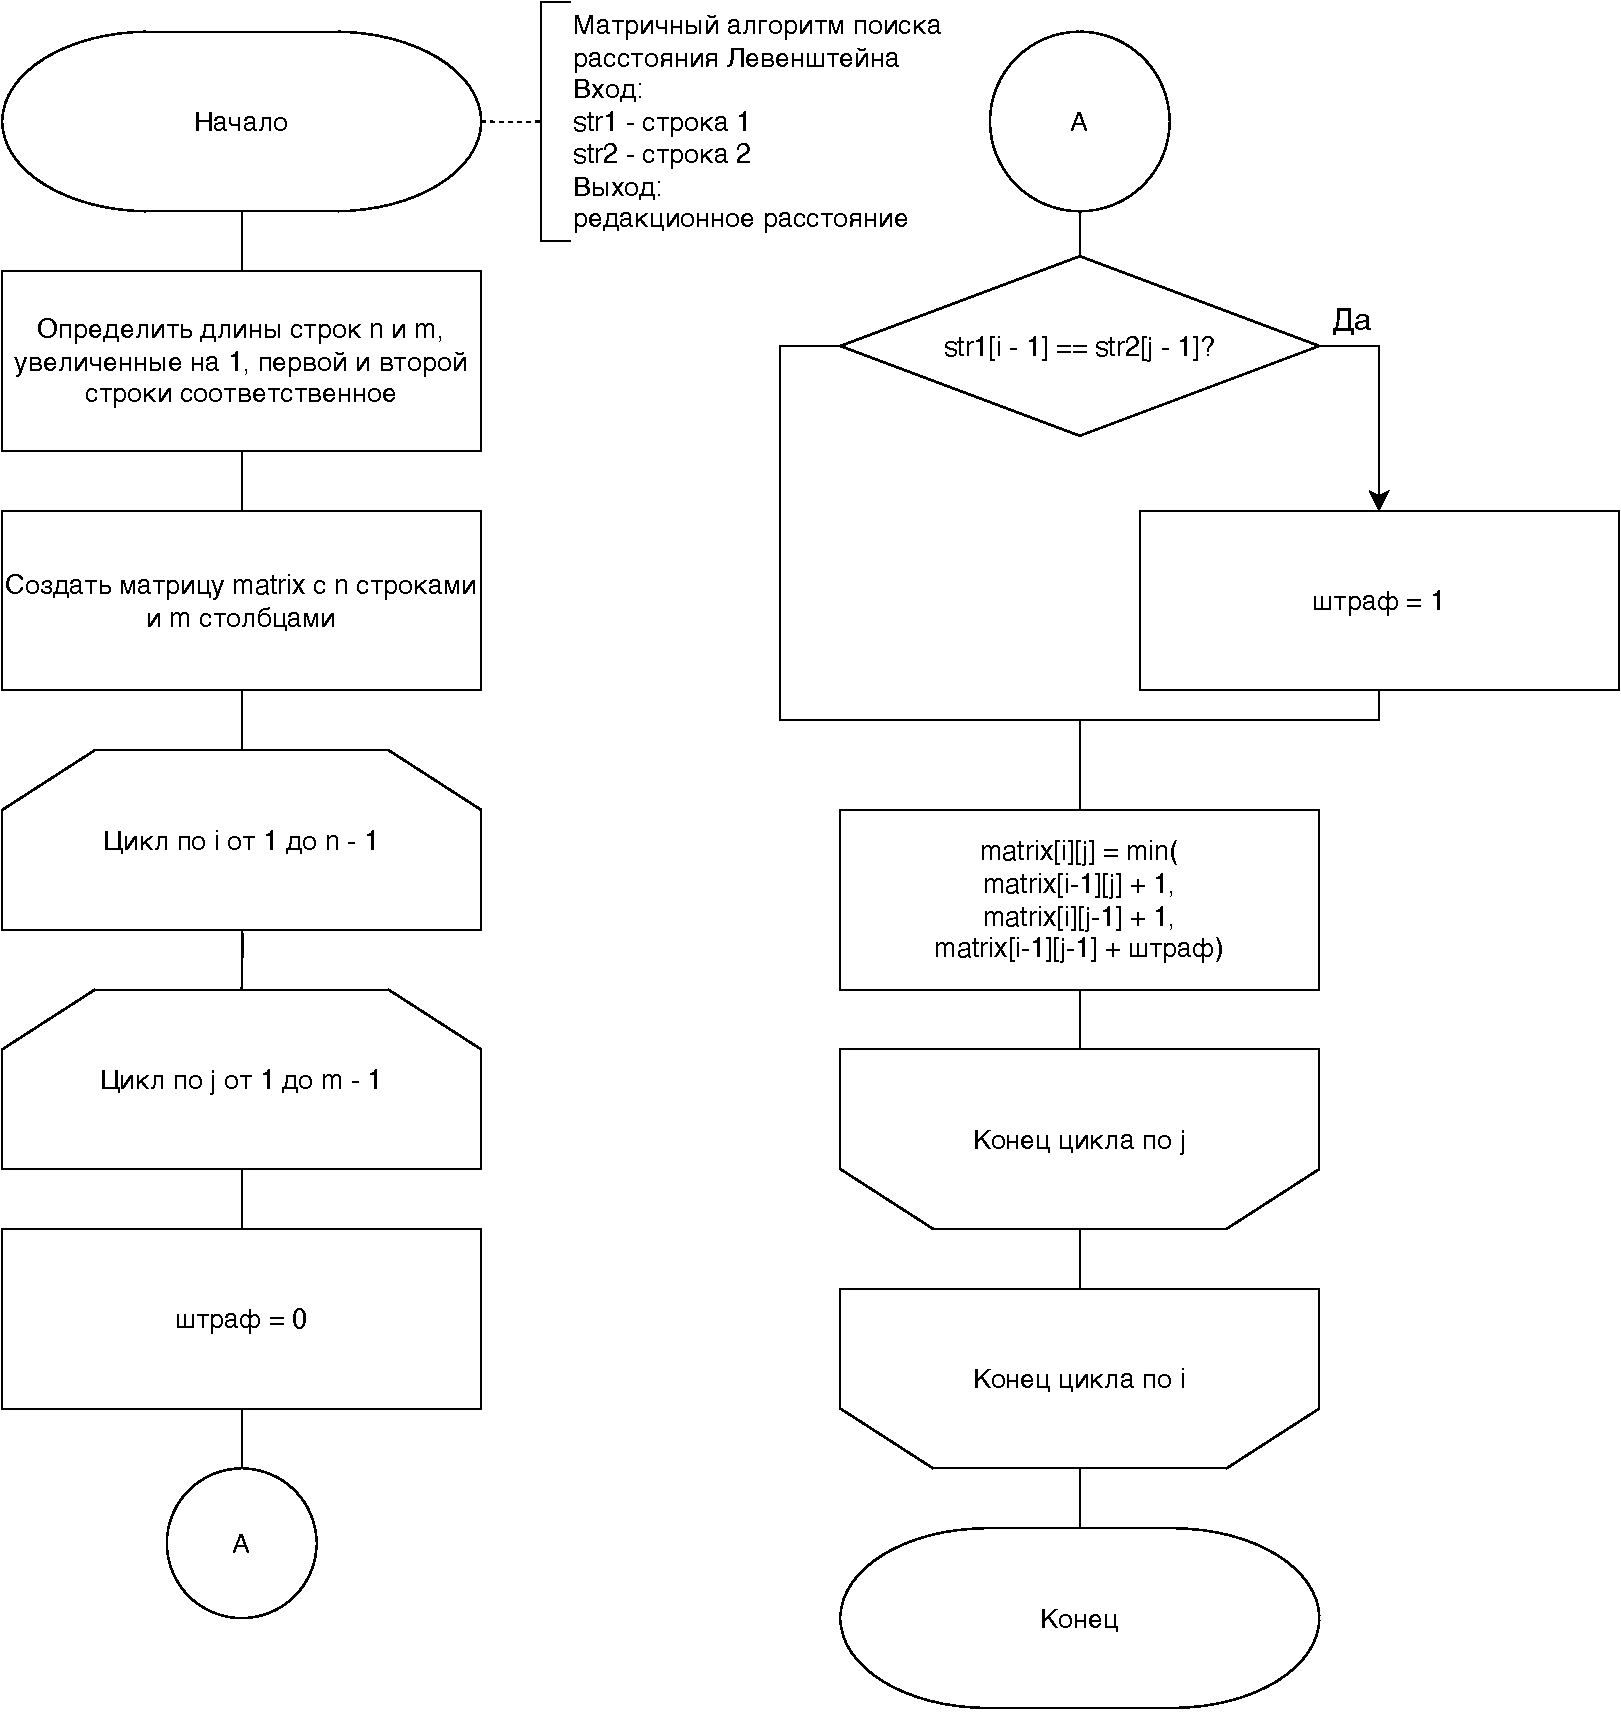
\includegraphics[scale=0.62]{assets/lev.pdf}
	\caption{Схема матричной реализации алгоритма поиска расстояния Левенштейна}
	\label{pic:lev}
\end{figure}

\section{Матричная реализация алгоритма поиска расстояния Дамерау---Левенштейна}

На рисунке \ref{pic:matr-dam-lev} приведена схема матричной реализации алгоритма поиска расстояния Дамерау---Левенштейна.

\newpage

\begin{figure}[H]
	\centering
	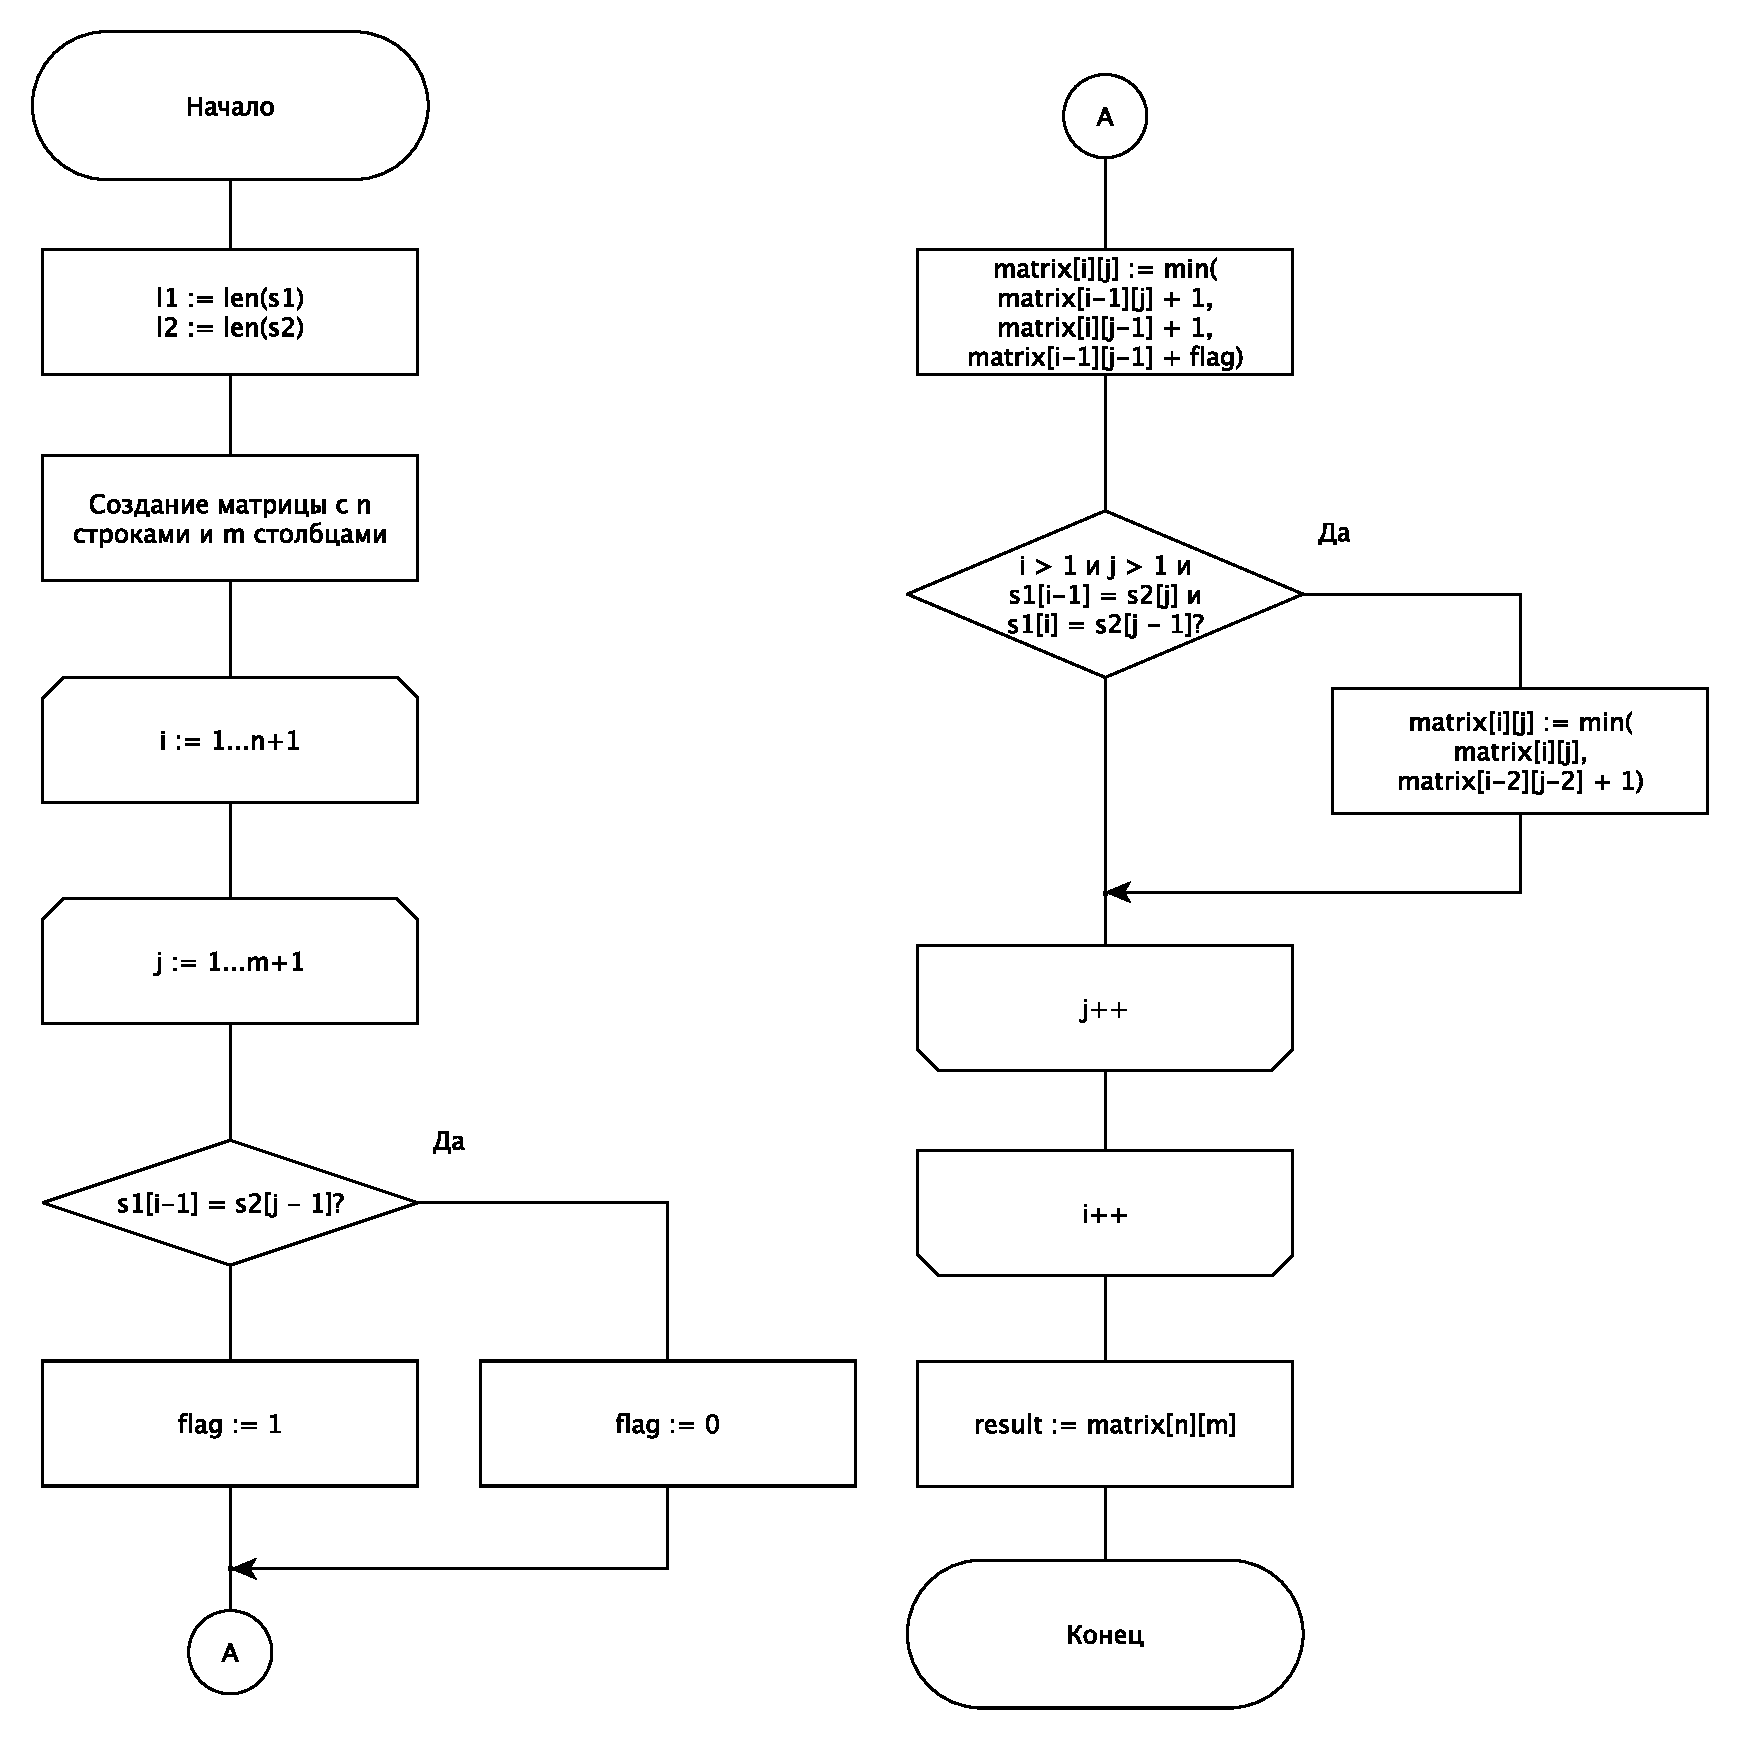
\includegraphics[scale=0.55]{assets/dam-lev-matr.pdf}
	\caption{Схема матричной реализации алгоритма поиска расстояния Дамерау---Левенштейна}
	\label{pic:matr-dam-lev}
\end{figure}

\section{Рекурсивная реализация алгоритма поиска расстояния Дамерау---Левенштейна}

На рисунке \ref{pic:rec-dam-lev} приведена схема рекурсивной реализации алгоритма поиска расстояния Дамерау---Левенштейна.

\begin{figure}[H]
	\centering
	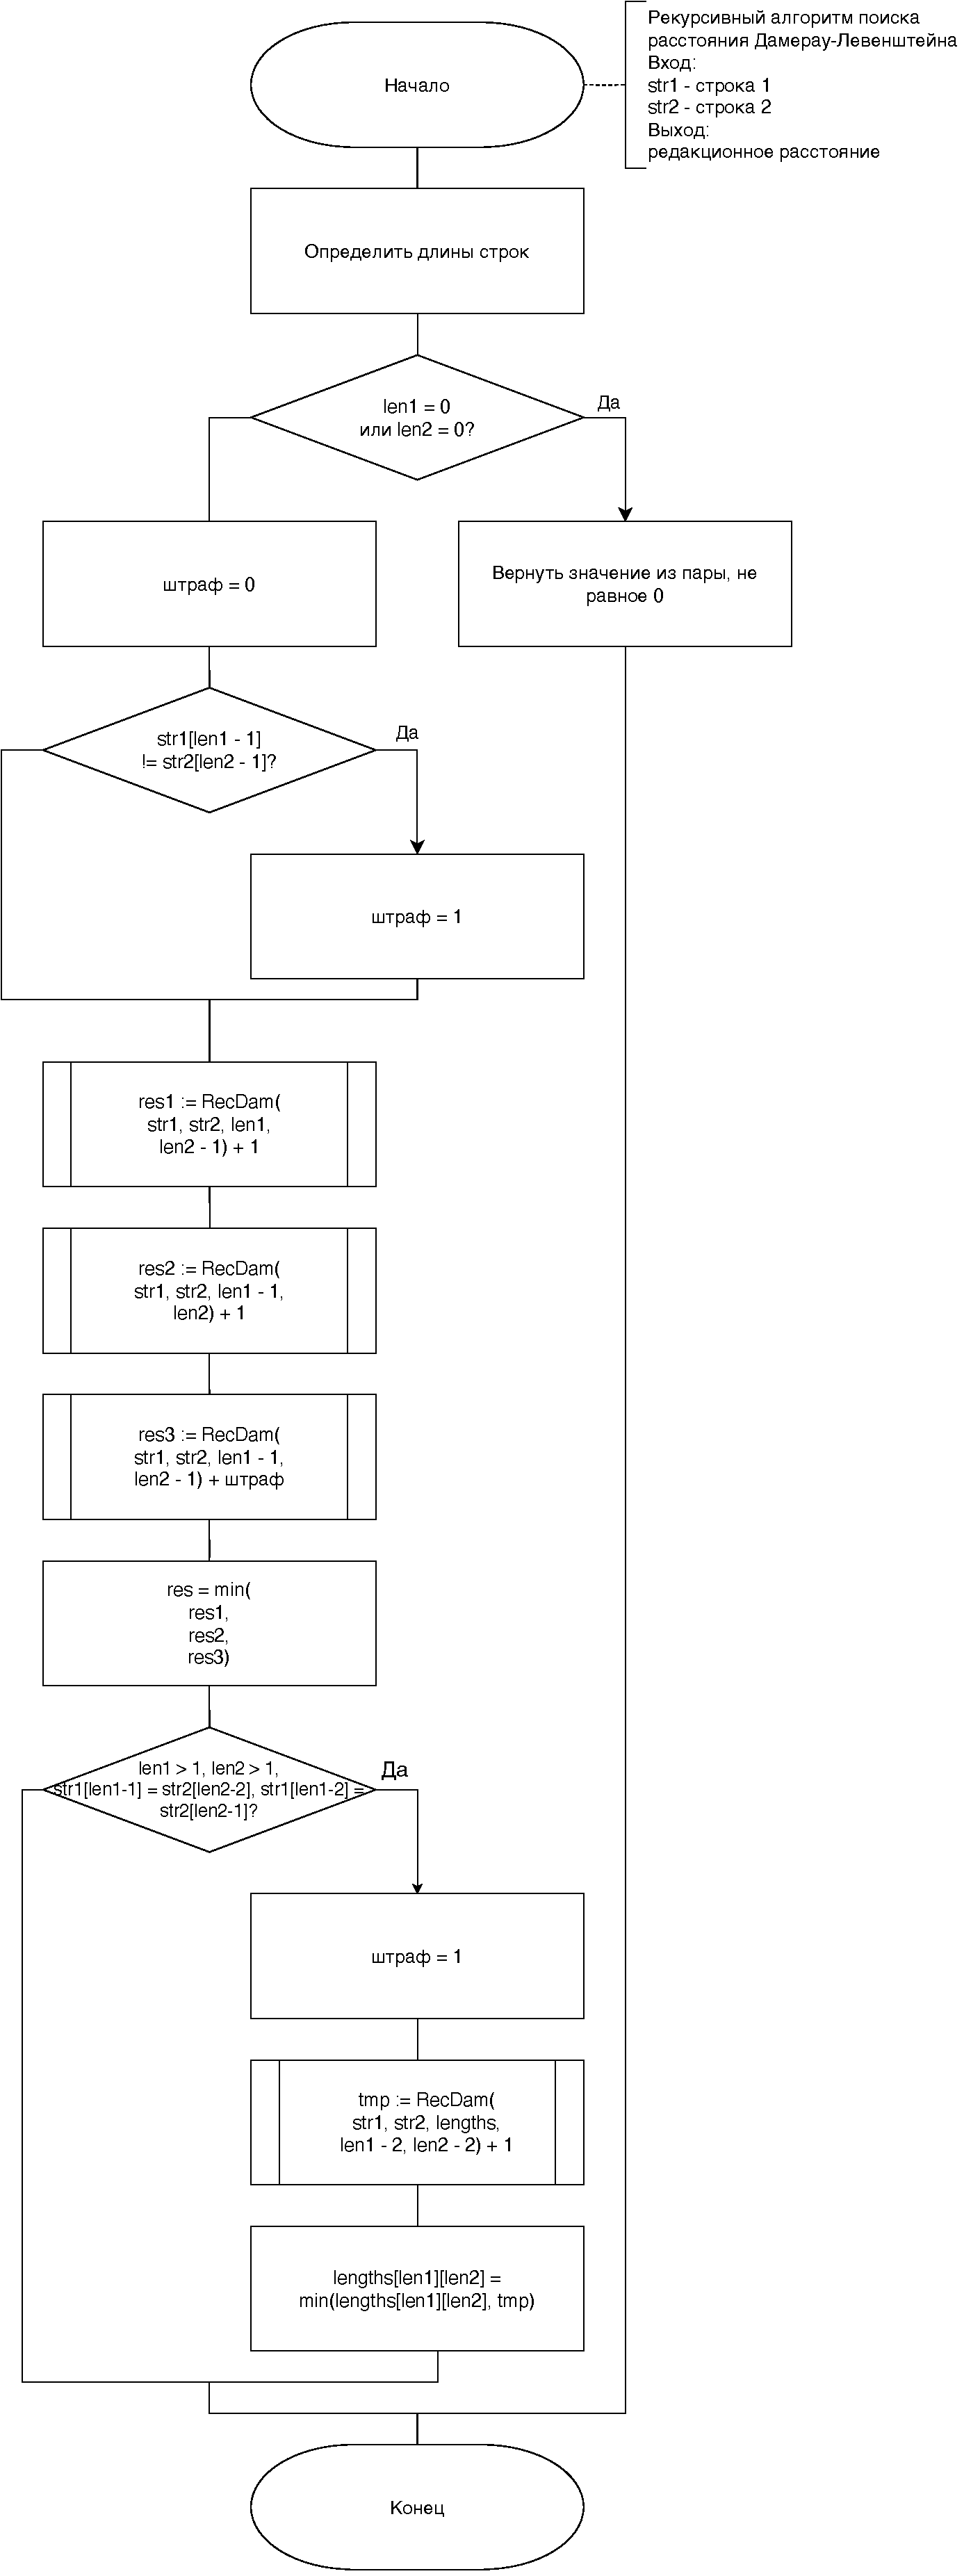
\includegraphics[scale=0.35]{assets/dam-lev-rec.pdf}
	\caption{Схема рекурсивной реализации алгоритма поиска расстояния Дамерау---Левенштейна}
	\label{pic:rec-dam-lev}
\end{figure}


\section{Рекурсивная реализация алгоритма поиска расстояния Дамерау---Левенштейна с кэшированием}

В качестве кэша используется матрица, инициализированная значениями <<-1>>. 

На рисунке \ref{pic:cache-dam-lev} приведена схема рекурсивной реализации алгоритма поиска расстояния Дамерау---Левенштейна с кэшированием.

\begin{figure}[H]
	\centering
	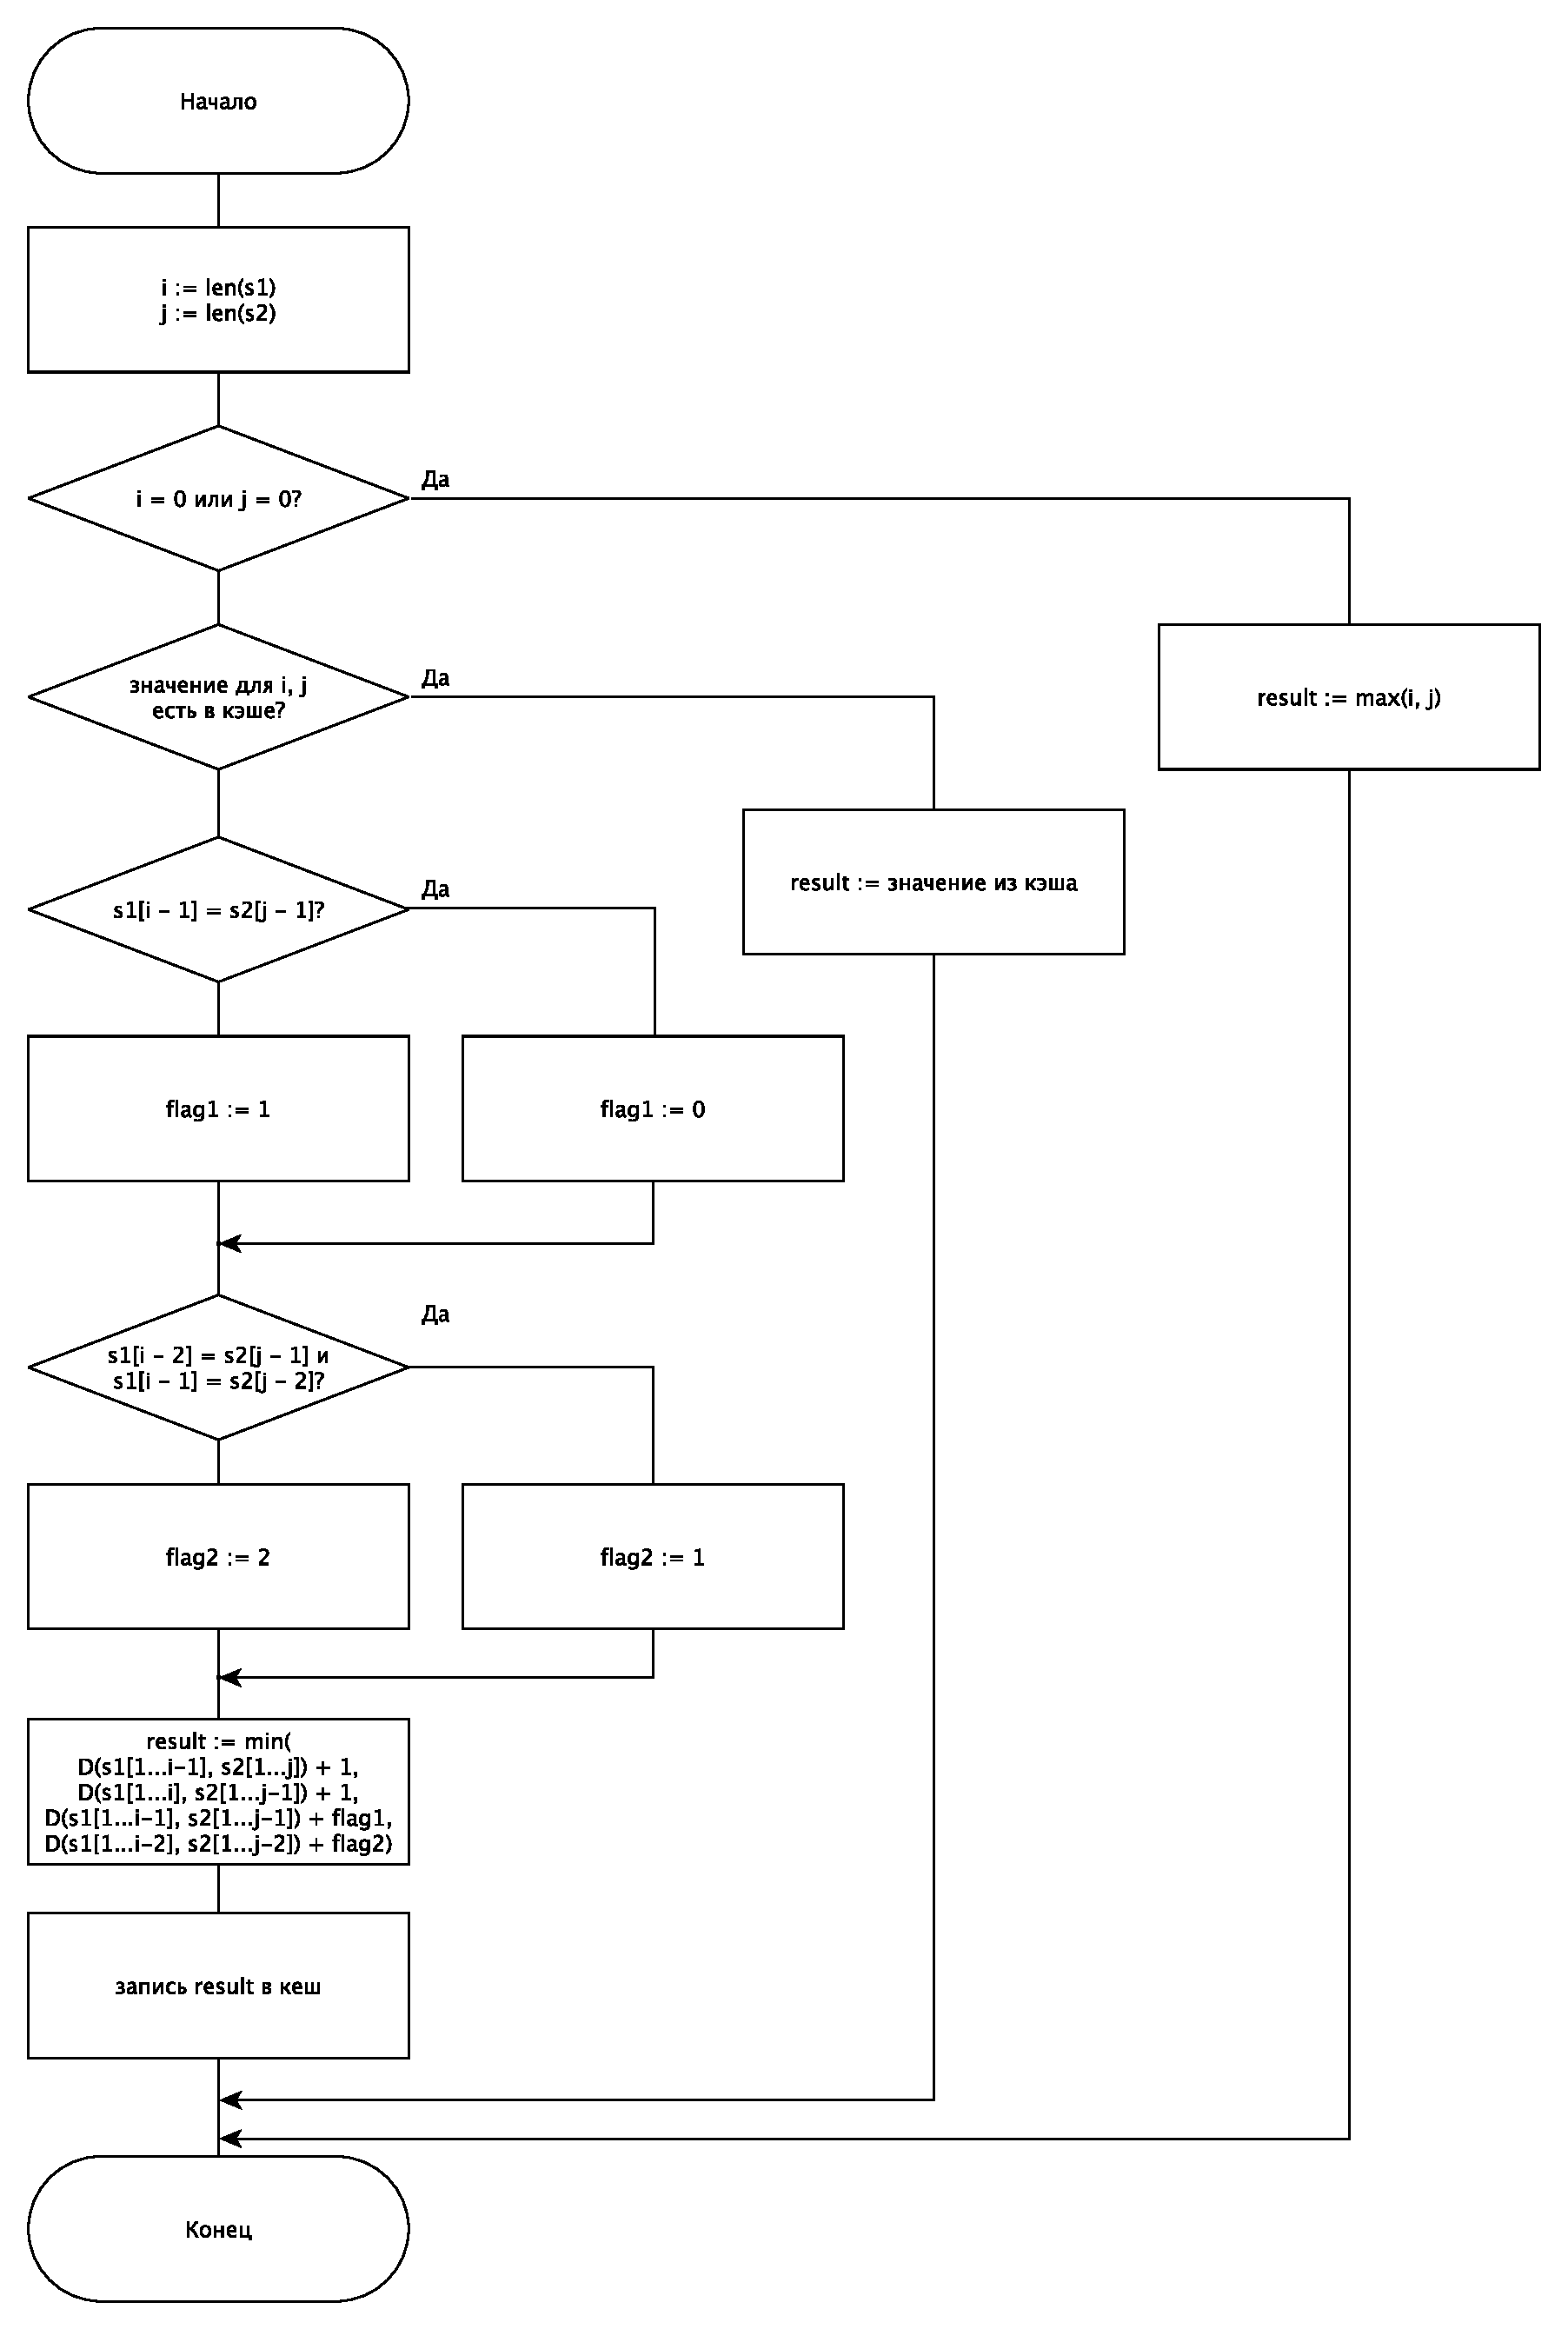
\includegraphics[scale=0.35]{assets/dam-lev-cache.pdf}
	\caption{Схема рекурсивной реализации алгоритма поиска расстояния Дамерау---Левенштейна с кэшированием}
	\label{pic:cache-dam-lev}
\end{figure}
